\chapter{Save data to File}
There are a lot of different ways to save data. Textfiles are simple to read, but less efficient when it comes to storage. Storing data in a binary format takes less storage, but the data is not readable by humans. A binary file is also less flexible when your data format might change. It is up to you to choose the right format for the job at hand.

\section{File Locations}
Whatever your choice, you will have to decide where to store the data. You could type in the full path in your code editor, but that's not a great idea.
Suppose you decide to save a config file to \verb|C:\myGame\gameData\config.txt.| This will be very anoying towards the user when she decides to save your app on another disk. It's even possible her computer does not even have a C drive!

Esenthel allows you to figure out some paths automatically. For example, you can retrieve the `documents' folder of the computer your app is running on:

\begin{code}
Str docPath = SystemPath(SP_DOCUMENTS);
\end{code}

When you'd like to save a file in the `documents' folder, it will be easy to construct the full path as:

\begin{code}
Str documentPath = S + docPath + "/myfile.txt";
\end{code} 

\begin{note}
You will be using the forward slash (/) in pathnames. Windows uses a backslash, but Esenthel will convert your forward slash when needed. This is because about every other operating system uses a forward slash in path names. To keep your project platform independent, always use forward slashes.
\end{note}

\verb|SP_DOCUMENTS| aside, there are some other system paths of use:

\begin{itemize}
\item \textbf{SP\_DESKTOP} will point to \verb|C:/Users/*/Desktop|.
\item \textbf{SP\_APP\_DATA} points to \verb|C:/Users/*/AppData/Roaming|. On a mobile device, this will be the location where the app is allowed to save data.
\item \textbf{SP\_APP\_DATA\_EXTERNAL} also refers \verb|C:/Users/*/AppData/Roaming|, but will point to an external SD card when your mobile device has one.
\item \textbf{SP\_ALL\_APP\_DATA} often refers to \verb|C:/ProgramData|
\end{itemize}

A complete list of possibilities can be found at \verb|Misc $\Rightarrow$ Misc|, below the enum declaration `SYSTEM\_PATH'. Not every path is available on every system though. You will not be able to write to the desktop of on a mobile platform.

\begin{exercise}
Find out where the paths on your computer point to. Create a simple test app which shows the different paths on the screen. \textsl{(Project Textfiles, ex. 01)}
\end{exercise}

\section{TextData}

The \eeClass{TextData} class is an easy way to store data as text. It's probably the best choice if you're looking to store a config file.

\subsection{Saving content}
You will uses `nodes' to store data. All data you consider worth saving must be assigned to a node. After assigning all data, the file must be saved to disk.

\begin{code}
TextData data;
data.getNode("name").setValue("John Doe");
data.getNode("highscore").setValue("100");
data.save(S + SystemPath(SP_DOCUMENTS) + "/config.txt");
\end{code} 

The method \eeFunc{getNode} will search for a node with a certain name. If no such node exists, a new one will be created. The method \eeFunc{setValue} will give the new node its value.

The resulting file will look like this:
\begin{verbatim}
name=`John Doe`
highscore=100
\end{verbatim}

\begin{exercise}
Create an app wit the variables \texttt{name}, \texttt{address}, and \texttt{age}. Assign default values to these variables and store them into a file. Open the file in a text editor and check these values.
\end{exercise}

\subsection{Loading a file}
\ldots goes like this:

\begin{code}
TextData data;
Str docPath = SystemPath(SP_DOCUMENTS);
data.load(S + docPath + "\config.txt");
\end{code}

If your documents folder has a file named `config.txt', it will be read. \textsl{(The function also returns a bool to indicate wether or not it succeeded. In a real application you should check its value.)}

\subsection{Reading content}
After loading a file, you can read its contents. To do this, you'll have to find the node you're looking for and assign its contents to a variable. Because it is possible that a certain node does not exist in your file, you should take two precautions:

\begin{enumerate}
	\item Assign a default value to all variables. When a node is not found, you still have the default value to work with.
	\item Only access a node when it exists. Accessing a node that does not exist will crash your application.
\end{enumerate}

\begin{code}
// config values
Str name = "new player";
int highScore = 0;
int credits = 100;

TextData data;
Str docPath = SystemPath(SP_DOCUMENTS);
if(data.load(S + docPath + "/config.txt")) {
   TextNode * node;
	 
	 // try finding the name
	 node = data.findNode("name");
	 if(node) {
	    name = node.asText();
	 }
	 
	 // try finding the highscore
	 node = data.findNode("highscore");
	 if(node) {
	    highScore = node.asInt();
	 }
}
\end{code}

\begin{note}
While saving a node, you can assign it about every value you want with the function\eeFunc{setValue}. But if you try to read it, you will have to tell the compiler what type of variable you're trying to read: you can use functions like \eeFunc{asInt} to load an integer, or \eeFunc{asText} vto load a string. More possibilities can be found in \verb|File $\Rightarrow$ Xml|. (\eeClass{TextNode} is based on \eeClass{TextParam}.)
\end{note}

\begin{exercise}
Adjust the generated file from the previous exercise in a text editor and load it back into your application. Show the values on the screen and double check to see if they are correct. \textsl{(Project Textfiles, ex. 02)}
\end{exercise}

\subsection{A class for a config file}
The following example is a complete class for your own config file. You should be able to adapt this to the needs of your own project. \textsl{(Project Textfiles, ex. 03)}

\begin{code}
class configFile {
private:
  Str name      = "new player";
	int highscore = 0  ;
	int credits   = 100;
	
public:
  Str getName     () { return name     ; }
	int getHighscore() { return highscore; }
	int getCredits  () { return credits  ; }
	
	void setName     (C Str & name   ) { T.name      = name   ; }
	void setHighscore(  int   score  ) { T.highscore = score  ; }
	void setCredits  (  int   credits) { T.credits   = credits; }
	
	void load() {
	  TextData data;
		if(data.load(S + SystemPath(SP_APP_DATA) + "/mygame/config.txt")) {
		  TextNode * node;
			
			if(node = data.findNode("name"     )) name      = node.asText();
			if(node = data.findNode("highscore")) highscore = node.asInt ();
			if(node = data.findNode("credits"  )) credits   = node.asInt ();
	  }
  }
	
	void save() {
	  TextData data;
		data.getNode("name"     ).setValue(name     );
		data.getNode("highscore").setValue(highscore);
		data.getNode("credits"  ).setValue(credits  );
		
		data.save(S + SystemPath(SP_APP_DATA) + "/mygame/config.txt");
  }
}
configFile ConfigFile;
\end{code}	

\section{Binary Files}
Files created with the class TextData are very useful for config files because you can change the contents with any text editor. But it's not the most efficient approach to store data. Data can be stored much more compact with the class \eeClass{File}. This class will store the data in a binary format, without an ID or any kind of internal structure to figure out what is what. The next example shows you how to open a file for writing and store several values in it. Note that this time, you have to specify the type you would like to store.

\begin{code}
File f;                  // create file object
f.write("file.dat"    ); // start writing to a file
f.putInt(128          ); // write an integer
f.putFlt(3.14         ); // write a float
f.putStr("Hello world"); // write a string
\end{code}

Reading data is similar. The function \eeFunc{readTry} will open the file for reading, if this is possible. If not, it will return false. \textsl{(A function \eeFunc{read} also exists, but when reading the data does not succeed, it will crash your application.)}

When you want to read data from a file, you will have to do this in the same order you stored it. Remember, the class \eeClass{file} has no clue what kind of data it is holding. 

\begin{code}
File f;
if (f.readTry("file.dat")) {
	int   i    = f.getInt();
	float pi   = f.getFlt();
	Str   text = f.getStr();
}
\end{code}

\begin{exercise}
Create a gui class with a \eeClass{TextLine}, a \eeClass{Slider}, a \eeClass{CheckBox} and two \eeClass{Button}s. The first button will save the current value of the gui elements on disk. The second button will load these values from disk and assigns them to the gui elements. Make sure to check if everything works like it should.
\end{exercise}

\subsection{Data Order}
But what happens if you read the contents of a file in another order you used while storing it? Look at this example:

\begin{code}
void save() {
  File f;
	f.write("trouble.dat");
	f.putBool(true);
	f.putInt (12  );
}

void load() {
  File f;
	f.read("trouble.dat");
	int i = f.getInt ();
	int b = f.getBool();
}
\end{code}

The save and load functions above do not use the same order for storing and reading. But the compiler will not alert you because there is no real error in the code as such. A bool variable is exactly 1 bit in size, and an integer takes 32 bits. In total 33 bits are stored: 1 + 32. But while reading the file, the code will ask for an integer first, and for a bool after that. So it will read 32 + 1 bits. That's still 33 bits! Only \ldots the values will be different from the ones you saved. Figure \ref{fig:filebits} illustrates this.

\begin{figure}[ht]
\centering
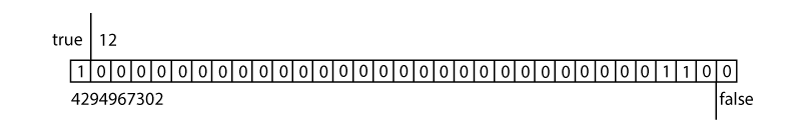
\includegraphics[width=0.8\linewidth]{../images/filebits}
\caption[]{bits in a file}
\label{fig:filebits}
\end{figure}

\begin{note}
The variable order while reading must match exactly with the order while saving. Unexpected behaviour will follow if it doesn't.
\end{note}

And there's another, less known, way in which things can go south. C++, like most programming languages, will handle function arguments from right to left. Most of the time we're not bothered by this. Take this code for example:
\begin{code}
float r = 0.1;
float x = 0.3;
float y = 0.4;

Circle c;
c.set(r, x, y);
\end{code}

If arguments are read from right to left, it means the instruction \eeFunc{pos2.set} happens in this order:

\begin{enumerate}
	\item Assign the value of y to the third argument of set.
	\item Assign the value of x to the second argument of set.
	\item Assign the value of r to the first argument of set.
	\item Execute whatever code is written inside set.
\end{enumerate}

We are not worried because it really doesn't matter in which order the data is being read. It's just there. The variables r, x and y can be read at any moment and they will always contain the right data.

The trouble starts when you read from a \textit{sequential} format. And yes, a binary file is a sequential format. So when you store these values to a file and read them like this\ldots

\begin{code}
float r = 0.1;
float x = 0.3;
float y = 0.4;

// Put data in an imaginary file
f.putFlt(r);
f.putFlt(x);
f.putFlt(y);

// ... after loading this data
Circle c;
c.set(f.getFlt(), f.getFlt(), f.getFlt());
\end{code}

\ldots you will be in for a big surprise (or at least a very confused coding session). Remember, the file contains the floats r, x and y. In that order.

When loading those floats in the last line of code, this is what happens:

\begin{enumerate}
\item The compiler sees that the third argument for set has to be retrieved from a file. "hey, give me a float", says the compiler to the file.
\item The file happily obliges and comes up with the first float in the data.
\item The compiler then finds out it needs another float, for the second argument. Again, a float is requested from the file.
\item The file, not having any clue what these floats are for, delivers the second float in the file.
\item You know what happens next. The third float in the file will be dumped as the first argument of set.
\end{enumerate}

To solve this sad misunderstanding between the compiler, the file and you, is is best to keep one thing in mind: don't retrieve more than one value from a file within a single argument list. In this particular case this means you don't use the set function.

\begin{code}
Circle c;
c.r     = f.getFlt();
c.pos.x = f.getFlt();
c.pos.y = f.getFlt();
\end{code}

\begin{exercise}
Now is your chance to do some evil programming. Abuse your skills to create a little program that demonstrates this error! \textsl{(Project Textfiles, ex. 04)}
\end{exercise}

\subsection{Storing multiple objects}
Sooner or later, you will want to store multiple objects in one file. There are several ways to do this, but as a rule of thumb two things will make your day easier.

\begin{enumerate}
	\item Before storing the actual object, store the number of objects that will follow.
	\item Create save and load methods for your object, and pass the current file as a reference.
\end{enumerate}

Below, you see a resource class with save and load methods. Notice that thes methods do not save or load any file directly. They merely add or read data to and from a file that will be created elsewhere.

\begin{code}
class resource {
  int type  ;
	Vec pos   ;
	int amount;
	
	void create(int type, int amount, C Vec & pos) {
	  T.type   = type  ;
		T.pos    = pos   ;
		T.amount = amount;
	}
	
	// ... other functions are omitted to keep this example short ...
	
	void save(File & f) {
	  f.putInt(type  );
		f.putFlt(pos.x ).putFlt(pos.y).putFlt(pos.z);
		f.putInt(amount);
	}
	
	void load(File & f) {
	  type   = f.getInt();
		pos.x  = f.getFlt();
		pos.y  = f.getFlt();
		pos.z  = f.getFlt();
		amount = f.getInt();
	}
}	
\end{code}

The next part is done by some sort of manager class. It has a container for resources (you've seen this concept before) and provides methods for saving and loading. 

This time, a file is opened. First the number of elements is written to the file. Afterwards, every resource is asked to write its own data to the same file.

\begin{code}
class resourceManager {
  Memx<resource> resources;
	
	void save() {
		File f;
		f.write("resources.dat");
		
		f.putInt(resources.elms());
		FREPA(resources) {
			resources[i].save(f);
		}
	}
	
	void load() {
	  File f;
		if(f.readTry("resources.dat")) {
			
			int elms = f.getInt();
			for(int i = 0; i < elms; i++) {
				resources.New().load(f);
			}
		}
	}
}

resourceManager RM;
\end{code}

When the file is loaded from disk, the number of stored resources is retrieved first. This is followed by a loop to create and load just as many resources as were stored in the file.

You can even go one step further and store every type of data in the same file, as long as you keep an eye of the order in which you write and read.

A program can call save functions for a resource manager, config file or anything you need, just by passing the file as a reference to every object with a save function. 

\begin{code}
void save() {
  File f;
	f.write("allData.data");
	Config.save(f);
	RM    .save(f);
}

void load() {
	File f;
	f.load("allData.data");
	Config.load(f);
	RM    .load(f);
}
\end{code}

\begin{note}
There is one drawback to this approach. When you update your software and add some new data, the new version of your application will not be able to read files written by the old version. Of course there are ways around this, but for now you'll just have to remember this limitation.
\end{note}

\begin{exercise}
Create a class for a circle that can remember its color. Create a manager class that can store these circles. Every mouseclick adds a circle to this manager, on the current mouse position. (Reread chapter \ref{section:managerClass} if you need help.)

When you close the application all circles are to be saved on disk. When the application starts, you must load all circles from the previous sessions.
\textsl{(Project Textfiles, ex. 05)}
\end{exercise}


